% Requires in LaTeX preamble:
% \usepackage{pgfplots}
% \usepgfplotslibrary{fillbetween}
% \pgfplotsset{compat=1.18}
\definecolor{expcolor0}{RGB}{76,114,176}
\definecolor{expcolor1}{RGB}{221,132,82}
\definecolor{expcolor2}{RGB}{85,168,104}
\begin{tikzpicture}
\begin{axis}[
xlabel={Steps ($\cdot 10^3$)},
ylabel={Computation time (s)},
axis lines=left,
xmin=0,
grid=both,
ymin=0,
]
\addplot[name path=pql_time_treasure_pressurelow, draw=none] coordinates {(2,0.3612001568) (4,0.9764383065) (6,1.544167338) (8,2.124542518) (10,2.765957364) (12,3.380832632) (14,4.008233656) (16,4.786052612) (18,5.478322005) (20,6.208320085) (22,7.000500477) (24,7.927240986) (26,8.665648286) (28,9.366864014) (30,10.15821665) (32,10.95603504) (34,11.77648607) (36,12.65229565) (38,13.51701926) (40,14.45816196) (42,15.27361086) (44,16.15217692) (46,17.05427139) (48,17.93230885) (50,18.90874784) (52,19.88296799) (54,20.89911166) (56,21.78849053) (58,22.68969268) (60,23.59570649) (62,24.58879396) (64,25.52936866) (66,26.57747385) (68,27.60371837) (70,28.45959214) (72,29.39258793) (74,30.31120867) (76,31.26917941) (78,32.23020924) (80,33.2026646) (82,34.16846767) (84,35.4296826) (86,36.4719103) (88,37.59578389) (90,38.77980367) (92,39.84922113) (94,40.83992106) (96,41.88844134) (98,43.04407304) (100,44.01299344) (102,45.0835942) (104,46.13898849) (106,47.29413147) (108,48.34417218) (110,49.36549293) (112,50.40349022) (114,51.44060796) (116,52.5268862) (118,53.59176036) (120,54.66610707) (122,55.7018759) (124,56.71831349) (126,57.70046689) (128,58.70705027) (130,59.81852174) (132,60.88989101) (134,61.92980037) (136,62.96101577) (138,63.97059396) (140,64.94885724) (142,65.96918471) (144,66.99880158) (146,68.08950948) (148,69.1145747) (150,70.13715147) (152,71.19600561) (154,72.37755145) (156,73.48044075) (158,74.52661464) (160,75.57684323) (162,76.78382903) (164,77.86603825) (166,79.05655965) (168,80.19518993) (170,81.25364815) (172,82.25602099) (174,83.35720207) (176,84.38236986) (178,85.38031284) (180,86.43549579) (182,87.39976714) (184,88.4266848) (186,89.4721937) (188,90.50938683) (190,91.49146252) (192,92.46019717) (194,93.51260822) (196,94.61555017) (198,95.6824054) (200,96.70880606)};
\addplot[name path=pql_time_treasure_pressureup, draw=none] coordinates {(2,0.4850879826) (4,1.049595097) (6,1.665123676) (8,2.252996113) (10,2.843310125) (12,3.56291612) (14,4.286781931) (16,5.020010417) (18,5.808432735) (20,6.493022553) (22,7.254420744) (24,7.99460793) (26,8.796070901) (28,9.955661102) (30,10.89938411) (32,11.83223622) (34,12.81485451) (36,13.82886427) (38,14.83251951) (40,15.82498478) (42,16.97108556) (44,18.02525002) (46,19.07309807) (48,20.07827947) (50,21.03453012) (52,22.00248171) (54,22.98420845) (56,24.04339062) (58,25.02195371) (60,26.03165799) (62,26.98479184) (64,27.98793989) (66,28.96974788) (68,29.96086275) (70,31.04173058) (72,32.00071181) (74,32.96889387) (76,33.99130381) (78,35.01291813) (80,36.01718433) (82,37.02851087) (84,38.00643733) (86,39.06746427) (88,40.01922333) (90,40.96599312) (92,41.9617804) (94,42.9620649) (96,43.97807477) (98,44.99158493) (100,46.08175952) (102,47.04046836) (104,48.03558404) (106,49.11176925) (108,50.11665266) (110,51.14768205) (112,52.15079848) (114,53.17007553) (116,54.28966427) (118,55.27192294) (120,56.28995772) (122,57.34114473) (124,58.35175604) (126,59.43236369) (128,60.48135711) (130,61.51311994) (132,62.64381094) (134,63.87536789) (136,64.96134235) (138,66.02227819) (140,67.14034015) (142,68.29331903) (144,69.33201743) (146,70.37514586) (148,71.50565969) (150,72.61544123) (152,73.65251666) (154,74.69085867) (156,75.78857357) (158,77.13524807) (160,78.52774642) (162,79.64878759) (164,80.88998217) (166,82.02788092) (168,83.1700119) (170,84.43769845) (172,85.6755896) (174,86.86608897) (176,88.12665603) (178,89.35992173) (180,90.7350532) (182,92.12921269) (184,93.51002262) (186,94.69309484) (188,95.93112773) (190,97.28207589) (192,98.81098299) (194,100.0002233) (196,101.267844) (198,102.4776937) (200,103.9432318)};
\addplot[draw=none, fill=expcolor0, fill opacity=0.15] fill between[of=pql_time_treasure_pressurelow and pql_time_treasure_pressureup];
\addplot[thick, draw=expcolor0] coordinates {(2,0.4231440697) (4,1.013016702) (6,1.604645507) (8,2.188769316) (10,2.804633744) (12,3.471874376) (14,4.147507793) (16,4.903031514) (18,5.64337737) (20,6.350671319) (22,7.12746061) (24,7.960924458) (26,8.730859594) (28,9.661262558) (30,10.52880038) (32,11.39413563) (34,12.29567029) (36,13.24057996) (38,14.17476939) (40,15.14157337) (42,16.12234821) (44,17.08871347) (46,18.06368473) (48,19.00529416) (50,19.97163898) (52,20.94272485) (54,21.94166005) (56,22.91594057) (58,23.8558232) (60,24.81368224) (62,25.7867929) (64,26.75865427) (66,27.77361087) (68,28.78229056) (70,29.75066136) (72,30.69664987) (74,31.64005127) (76,32.63024161) (78,33.62156368) (80,34.60992446) (82,35.59848927) (84,36.71805996) (86,37.76968729) (88,38.80750361) (90,39.8728984) (92,40.90550076) (94,41.90099298) (96,42.93325805) (98,44.01782899) (100,45.04737648) (102,46.06203128) (104,47.08728626) (106,48.20295036) (108,49.23041242) (110,50.25658749) (112,51.27714435) (114,52.30534174) (116,53.40827523) (118,54.43184165) (120,55.47803239) (122,56.52151031) (124,57.53503476) (126,58.56641529) (128,59.59420369) (130,60.66582084) (132,61.76685098) (134,62.90258413) (136,63.96117906) (138,64.99643608) (140,66.04459869) (142,67.13125187) (144,68.1654095) (146,69.23232767) (148,70.31011719) (150,71.37629635) (152,72.42426114) (154,73.53420506) (156,74.63450716) (158,75.83093135) (160,77.05229482) (162,78.21630831) (164,79.37801021) (166,80.54222029) (168,81.68260091) (170,82.8456733) (172,83.96580529) (174,85.11164552) (176,86.25451295) (178,87.37011728) (180,88.58527449) (182,89.76448992) (184,90.96835371) (186,92.08264427) (188,93.22025728) (190,94.38676921) (192,95.63559008) (194,96.75641576) (196,97.94169707) (198,99.08004957) (200,100.3260189)};
\addplot[name path=pqlrm_time_treasure_pressurelow, draw=none] coordinates {(2,1.90932172) (4,4.152735574) (6,6.61165667) (8,9.194419875) (10,11.92882114) (12,14.98437991) (14,17.72283849) (16,20.3693437) (18,23.1173255) (20,25.80555466) (22,28.70189515) (24,31.71882761) (26,34.87688549) (28,37.91138594) (30,40.92128815) (32,43.87155767) (34,47.0835077) (36,50.36203215) (38,53.61311253) (40,56.81993059) (42,60.0612175) (44,63.38554956) (46,66.55213908) (48,69.67837354) (50,72.79664033) (52,75.93720194) (54,79.10217142) (56,82.32431911) (58,85.43950218) (60,88.56158239) (62,91.76987901) (64,94.89696955) (66,98.01237684) (68,101.2141681) (70,104.3461006) (72,107.4309203) (74,110.5820564) (76,113.7083865) (78,116.8613274) (80,119.9601616) (82,123.1143666) (84,126.2453239) (86,129.3476236) (88,132.4371015) (90,135.5698736) (92,138.741633) (94,141.8359382) (96,145.0302175) (98,148.1450479) (100,151.2805939) (102,151.2805939) (104,151.2805939) (106,151.2805939) (108,151.2805939) (110,151.2805939) (112,151.2805939) (114,151.2805939) (116,151.2805939) (118,151.2805939) (120,151.2805939) (122,151.2805939) (124,151.2805939) (126,151.2805939) (128,151.2805939) (130,151.2805939) (132,151.2805939) (134,151.2805939) (136,151.2805939) (138,151.2805939) (140,151.2805939) (142,151.2805939) (144,151.2805939) (146,151.2805939) (148,151.2805939) (150,151.2805939) (152,151.2805939) (154,151.2805939) (156,151.2805939) (158,151.2805939) (160,151.2805939) (162,151.2805939) (164,151.2805939) (166,151.2805939) (168,151.2805939) (170,151.2805939) (172,151.2805939) (174,151.2805939) (176,151.2805939) (178,151.2805939) (180,151.2805939) (182,151.2805939) (184,151.2805939) (186,151.2805939) (188,151.2805939) (190,151.2805939) (192,151.2805939) (194,151.2805939) (196,151.2805939) (198,151.2805939) (200,151.2805939)};
\addplot[name path=pqlrm_time_treasure_pressureup, draw=none] coordinates {(2,2.223106288) (4,4.734443097) (6,7.26085376) (8,9.713371411) (10,12.3579687) (12,15.10783348) (14,18.17180478) (16,21.26337639) (18,24.2183633) (20,27.33293395) (22,30.30509617) (24,33.16845256) (26,36.18859545) (28,39.49944426) (30,42.90737076) (32,46.35966133) (34,49.77227216) (36,52.95146772) (38,56.16128733) (40,59.54809999) (42,62.75122846) (44,65.96458474) (46,69.2038199) (48,72.36848629) (50,75.63972232) (52,78.93782561) (54,82.22267348) (56,85.37261704) (58,88.5422227) (60,91.7114714) (62,94.92319319) (64,98.1989044) (66,101.5556488) (68,104.7208456) (70,107.8956285) (72,111.1297463) (74,114.2604193) (76,117.4473759) (78,120.575545) (80,123.7709928) (82,126.9241488) (84,130.1098071) (86,133.2834606) (88,136.4656626) (90,139.654795) (92,142.8499409) (94,146.1355418) (96,149.2736075) (98,152.4394582) (100,155.5943877) (102,155.5943877) (104,155.5943877) (106,155.5943877) (108,155.5943877) (110,155.5943877) (112,155.5943877) (114,155.5943877) (116,155.5943877) (118,155.5943877) (120,155.5943877) (122,155.5943877) (124,155.5943877) (126,155.5943877) (128,155.5943877) (130,155.5943877) (132,155.5943877) (134,155.5943877) (136,155.5943877) (138,155.5943877) (140,155.5943877) (142,155.5943877) (144,155.5943877) (146,155.5943877) (148,155.5943877) (150,155.5943877) (152,155.5943877) (154,155.5943877) (156,155.5943877) (158,155.5943877) (160,155.5943877) (162,155.5943877) (164,155.5943877) (166,155.5943877) (168,155.5943877) (170,155.5943877) (172,155.5943877) (174,155.5943877) (176,155.5943877) (178,155.5943877) (180,155.5943877) (182,155.5943877) (184,155.5943877) (186,155.5943877) (188,155.5943877) (190,155.5943877) (192,155.5943877) (194,155.5943877) (196,155.5943877) (198,155.5943877) (200,155.5943877)};
\addplot[draw=none, fill=expcolor1, fill opacity=0.15] fill between[of=pqlrm_time_treasure_pressurelow and pqlrm_time_treasure_pressureup];
\addplot[thick, draw=expcolor1] coordinates {(2,2.066214004) (4,4.443589335) (6,6.936255215) (8,9.453895643) (10,12.14339492) (12,15.0461067) (14,17.94732163) (16,20.81636004) (18,23.6678444) (20,26.5692443) (22,29.50349566) (24,32.44364008) (26,35.53274047) (28,38.7054151) (30,41.91432945) (32,45.1156095) (34,48.42788993) (36,51.65674994) (38,54.88719993) (40,58.18401529) (42,61.40622298) (44,64.67506715) (46,67.87797949) (48,71.02342992) (50,74.21818132) (52,77.43751377) (54,80.66242245) (56,83.84846807) (58,86.99086244) (60,90.1365269) (62,93.3465361) (64,96.54793698) (66,99.78401282) (68,102.9675068) (70,106.1208646) (72,109.2803333) (74,112.4212379) (76,115.5778812) (78,118.7184362) (80,121.8655772) (82,125.0192577) (84,128.1775655) (86,131.3155421) (88,134.4513821) (90,137.6123343) (92,140.795787) (94,143.98574) (96,147.1519125) (98,150.292253) (100,153.4374908) (102,153.4374908) (104,153.4374908) (106,153.4374908) (108,153.4374908) (110,153.4374908) (112,153.4374908) (114,153.4374908) (116,153.4374908) (118,153.4374908) (120,153.4374908) (122,153.4374908) (124,153.4374908) (126,153.4374908) (128,153.4374908) (130,153.4374908) (132,153.4374908) (134,153.4374908) (136,153.4374908) (138,153.4374908) (140,153.4374908) (142,153.4374908) (144,153.4374908) (146,153.4374908) (148,153.4374908) (150,153.4374908) (152,153.4374908) (154,153.4374908) (156,153.4374908) (158,153.4374908) (160,153.4374908) (162,153.4374908) (164,153.4374908) (166,153.4374908) (168,153.4374908) (170,153.4374908) (172,153.4374908) (174,153.4374908) (176,153.4374908) (178,153.4374908) (180,153.4374908) (182,153.4374908) (184,153.4374908) (186,153.4374908) (188,153.4374908) (190,153.4374908) (192,153.4374908) (194,153.4374908) (196,153.4374908) (198,153.4374908) (200,153.4374908)};
\addplot[name path=qrm_time_treasure_pressurelow, draw=none] coordinates {(2,0.1820210286) (4,0.3752223266) (6,0.5712155791) (8,0.7601581292) (10,0.9518971301) (12,1.135759163) (14,1.321336886) (16,1.508651957) (18,1.694429141) (20,1.867858742) (22,2.052316508) (24,2.229143262) (26,2.407170687) (28,2.588468521) (30,2.764313958) (32,2.949165866) (34,3.126683757) (36,3.306371572) (38,3.542417283) (40,3.49935847) (42,3.49935847) (44,3.49935847) (46,3.49935847) (48,3.49935847) (50,3.49935847) (52,3.49935847) (54,3.49935847) (56,3.49935847) (58,3.49935847) (60,3.49935847) (62,3.49935847) (64,3.49935847) (66,3.49935847) (68,3.49935847) (70,3.49935847) (72,3.49935847) (74,3.49935847) (76,3.49935847) (78,3.49935847) (80,3.49935847) (82,3.49935847) (84,3.49935847) (86,3.49935847) (88,3.49935847) (90,3.49935847) (92,3.49935847) (94,3.49935847) (96,3.49935847) (98,3.49935847) (100,3.49935847) (102,3.49935847) (104,3.49935847) (106,3.49935847) (108,3.49935847) (110,3.49935847) (112,3.49935847) (114,3.49935847) (116,3.49935847) (118,3.49935847) (120,3.49935847) (122,3.49935847) (124,3.49935847) (126,3.49935847) (128,3.49935847) (130,3.49935847) (132,3.49935847) (134,3.49935847) (136,3.49935847) (138,3.49935847) (140,3.49935847) (142,3.49935847) (144,3.49935847) (146,3.49935847) (148,3.49935847) (150,3.49935847) (152,3.49935847) (154,3.49935847) (156,3.49935847) (158,3.49935847) (160,3.49935847) (162,3.49935847) (164,3.49935847) (166,3.49935847) (168,3.49935847) (170,3.49935847) (172,3.49935847) (174,3.49935847) (176,3.49935847) (178,3.49935847) (180,3.49935847) (182,3.49935847) (184,3.49935847) (186,3.49935847) (188,3.49935847) (190,3.49935847) (192,3.49935847) (194,3.49935847) (196,3.49935847) (198,3.49935847) (200,3.49935847)};
\addplot[name path=qrm_time_treasure_pressureup, draw=none] coordinates {(2,0.1910940074) (4,0.3858681454) (6,0.6090308956) (8,0.8054322555) (10,0.9973106565) (12,1.200259492) (14,1.406309827) (16,1.61030868) (18,1.815744471) (20,2.076585928) (22,2.272306096) (24,2.467586394) (26,2.656656373) (28,2.837836642) (30,3.02451671) (32,3.211016325) (34,3.390627776) (36,3.568823028) (38,3.572210763) (40,3.737747668) (42,3.737747668) (44,3.737747668) (46,3.737747668) (48,3.737747668) (50,3.737747668) (52,3.737747668) (54,3.737747668) (56,3.737747668) (58,3.737747668) (60,3.737747668) (62,3.737747668) (64,3.737747668) (66,3.737747668) (68,3.737747668) (70,3.737747668) (72,3.737747668) (74,3.737747668) (76,3.737747668) (78,3.737747668) (80,3.737747668) (82,3.737747668) (84,3.737747668) (86,3.737747668) (88,3.737747668) (90,3.737747668) (92,3.737747668) (94,3.737747668) (96,3.737747668) (98,3.737747668) (100,3.737747668) (102,3.737747668) (104,3.737747668) (106,3.737747668) (108,3.737747668) (110,3.737747668) (112,3.737747668) (114,3.737747668) (116,3.737747668) (118,3.737747668) (120,3.737747668) (122,3.737747668) (124,3.737747668) (126,3.737747668) (128,3.737747668) (130,3.737747668) (132,3.737747668) (134,3.737747668) (136,3.737747668) (138,3.737747668) (140,3.737747668) (142,3.737747668) (144,3.737747668) (146,3.737747668) (148,3.737747668) (150,3.737747668) (152,3.737747668) (154,3.737747668) (156,3.737747668) (158,3.737747668) (160,3.737747668) (162,3.737747668) (164,3.737747668) (166,3.737747668) (168,3.737747668) (170,3.737747668) (172,3.737747668) (174,3.737747668) (176,3.737747668) (178,3.737747668) (180,3.737747668) (182,3.737747668) (184,3.737747668) (186,3.737747668) (188,3.737747668) (190,3.737747668) (192,3.737747668) (194,3.737747668) (196,3.737747668) (198,3.737747668) (200,3.737747668)};
\addplot[draw=none, fill=expcolor2, fill opacity=0.15] fill between[of=qrm_time_treasure_pressurelow and qrm_time_treasure_pressureup];
\addplot[thick, draw=expcolor2] coordinates {(2,0.186557518) (4,0.380545236) (6,0.5901232373) (8,0.7827951923) (10,0.9746038933) (12,1.168009328) (14,1.363823357) (16,1.559480319) (18,1.755086806) (20,1.972222335) (22,2.162311302) (24,2.348364828) (26,2.53191353) (28,2.713152581) (30,2.894415334) (32,3.080091095) (34,3.258655766) (36,3.4375973) (38,3.557314023) (40,3.618553069) (42,3.618553069) (44,3.618553069) (46,3.618553069) (48,3.618553069) (50,3.618553069) (52,3.618553069) (54,3.618553069) (56,3.618553069) (58,3.618553069) (60,3.618553069) (62,3.618553069) (64,3.618553069) (66,3.618553069) (68,3.618553069) (70,3.618553069) (72,3.618553069) (74,3.618553069) (76,3.618553069) (78,3.618553069) (80,3.618553069) (82,3.618553069) (84,3.618553069) (86,3.618553069) (88,3.618553069) (90,3.618553069) (92,3.618553069) (94,3.618553069) (96,3.618553069) (98,3.618553069) (100,3.618553069) (102,3.618553069) (104,3.618553069) (106,3.618553069) (108,3.618553069) (110,3.618553069) (112,3.618553069) (114,3.618553069) (116,3.618553069) (118,3.618553069) (120,3.618553069) (122,3.618553069) (124,3.618553069) (126,3.618553069) (128,3.618553069) (130,3.618553069) (132,3.618553069) (134,3.618553069) (136,3.618553069) (138,3.618553069) (140,3.618553069) (142,3.618553069) (144,3.618553069) (146,3.618553069) (148,3.618553069) (150,3.618553069) (152,3.618553069) (154,3.618553069) (156,3.618553069) (158,3.618553069) (160,3.618553069) (162,3.618553069) (164,3.618553069) (166,3.618553069) (168,3.618553069) (170,3.618553069) (172,3.618553069) (174,3.618553069) (176,3.618553069) (178,3.618553069) (180,3.618553069) (182,3.618553069) (184,3.618553069) (186,3.618553069) (188,3.618553069) (190,3.618553069) (192,3.618553069) (194,3.618553069) (196,3.618553069) (198,3.618553069) (200,3.618553069)};
\end{axis}
\end{tikzpicture}
% Manual legend fallback with explicit colored lines:
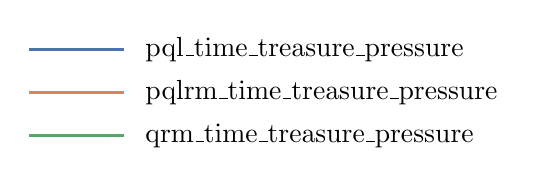
\begin{tikzpicture}
\draw[very thick, draw=expcolor0] (1.00,0.00) -- (2.20,0.00);
\node[anchor=west] at (2.35,0.00) {pql\_time\_treasure\_pressure};
\draw[very thick, draw=expcolor1] (1.00,-0.55) -- (2.20,-0.55);
\node[anchor=west] at (2.35,-0.55) {pqlrm\_time\_treasure\_pressure};
\draw[very thick, draw=expcolor2] (1.00,-1.10) -- (2.20,-1.10);
\node[anchor=west] at (2.35,-1.10) {qrm\_time\_treasure\_pressure};
\end{tikzpicture}
% caption: Computation Time - pbst\_exp1, with 95\textbackslash\{\}\% uncertainty bands.
